\documentclass[fleqn]{article}
\oddsidemargin 0.0in
\textwidth 6.0in
\thispagestyle{empty}
\usepackage{import}
\usepackage{amsmath}
\usepackage{amssymb}
\usepackage{graphicx}
\usepackage[english]{babel}
\usepackage[utf8x]{inputenc}
\usepackage{float}
\usepackage{bigints} 
\usepackage[colorinlistoftodos]{todonotes}
\usepackage{setspace}
\usepackage{geometry}
\usepackage{colortbl}
\usepackage{xcolor,colortbl}


\newcommand{\va}{\mbox{\boldmath{$a$}}}
\newcommand{\vb}{\mbox{\boldmath{$b$}}}
\newcommand{\vc}{\mbox{\boldmath{$c$}}}
\newcommand{\vd}{\mbox{\boldmath{$d$}}}
\newcommand{\vi}{\mbox{\boldmath{$i$}}}
\newcommand{\vj}{\mbox{\boldmath{$j$}}}
\newcommand{\vk}{\mbox{\boldmath{$k$}}}
\newcommand{\vr}{\mbox{\boldmath{$r$}}}
\newcommand{\vectr}[1]{\mbox{\boldmath{${#1}$}}}
\newcommand{\unitvec}[1]{\mbox{\boldmath{$\hat{#1}$}}}
\newcommand{\matA}{\mbox{$\underline{\underline{A}}$}}
\newcommand{\matB}{\mbox{$\underline{\underline{B}}$}}
\newcommand{\matAtranspose}{\mbox{$\underline{\underline{\tilde{A}}}$}}
\newcommand{\matBtranspose}{\mbox{$\underline{\underline{\tilde{B}}}$}}
\newcommand{\matone}{$\underline{\underline{I}}$}
\newcommand{\grad}[1]{\mbox{\boldmath $\nabla$}\mbox{$#1$}}
\newcommand{\divg}[1]{\mbox{\boldmath $\nabla$} \mbox{$\cdot$} \mbox{\boldmath $#1$}}
\newcommand{\curl}[1]{\mbox{\boldmath $\nabla$} \mbox{$\times$} \mbox{\boldmath $#1$}}
\newcommand{\prtl}[2]{\ensuremath{\frac{\partial #1}{\partial #2}}}
\newcommand{\prtll}[2]{\ensuremath{\frac{\partial^{2} #1}{\partial {#2}^{2}}}}
\newcommand{\yd}[2]{\ensuremath{\frac{d #1}{d #2}}}
\newcommand{\ydd}[2]{\ensuremath{\frac{d^{2} #1}{d {#2}^{2}}}}

\definecolor{hwColor}{HTML}{AD53BA}
\definecolor{contents}{HTML}{EAFF7C}
\definecolor{red}{HTML}{FF0000}

\doublespacing
\begin{document}

\begin{titlepage}

\newcommand{\HRule}{\rule{\linewidth}{0.5mm}}

\center
 

\textsc{\LARGE Arizona State University}\\[1.5cm] 

\textsc{\LARGE Mathematical Methods For Physics II }\\[1.5cm]


\begin{figure}
  
\includegraphics[width=\linewidth]{asu.png}
\end{figure}


\HRule \\[0.4cm]
{ \huge \bfseries Portfolio}\\[0.4cm] 
\HRule \\[1.5cm]
 
\textbf{Behnam Amiri}

\bigbreak

\textbf{Prof: Cecilia Lunardini (Grader. Kenna McRae)}

\bigbreak


\textbf{{\large \today}\\[2cm]}

\vfill

\end{titlepage}

\huge \textbf{Academic integrity statement:}

\bigbreak

\Large I am aware of the course rules detailed in the syllabus and related course documents. I am also aware of Arizona State University’s policies and practices against plagiarism and other forms of academic dishonesty. I affirm that I have not given or received any unauthorized help on this assignment, and I have not used any unauthorized resources. All authorized help (from the instructor, or learning assistant), authorized collaborations (with classmates), and authorized resources are explicitly stated and described in detail in the present document.

\bigbreak

\Large This work is entirely my own, except when collaboration with classmates is explicitly declared, and I take full responsibility for it.

\bigbreak

\Large Signature and date:

\bigbreak

\bigbreak


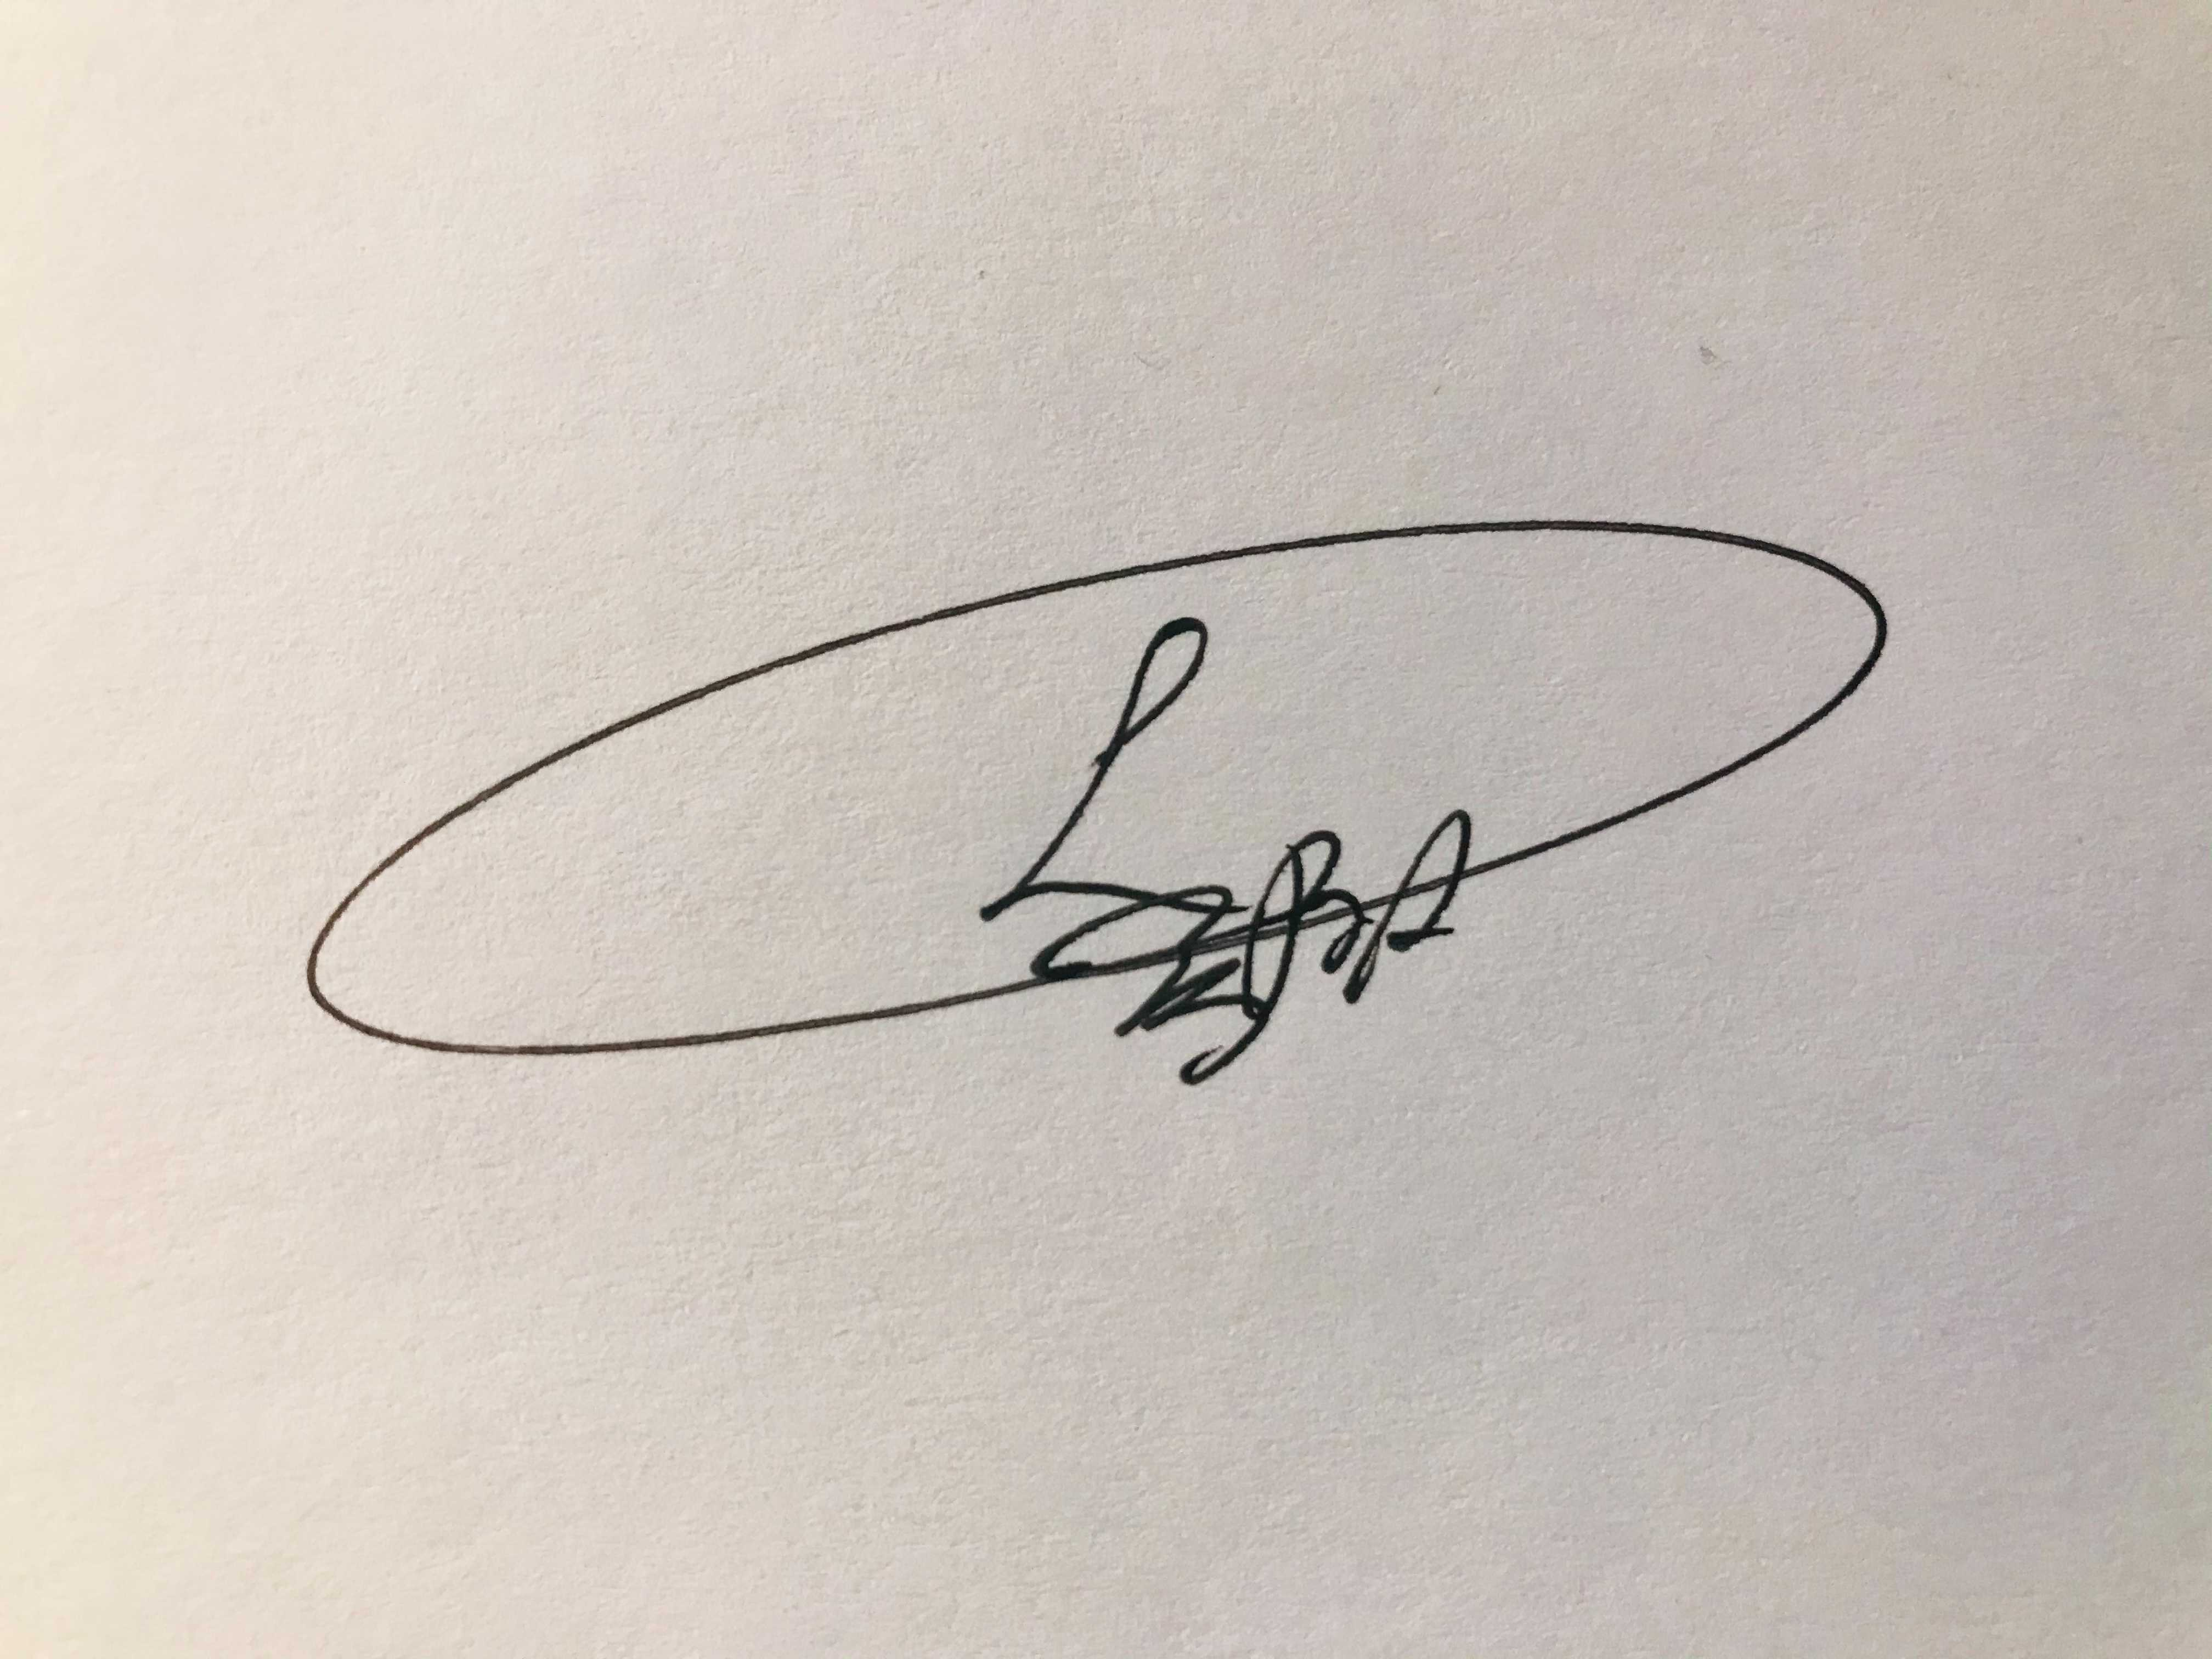
\includegraphics[height=3cm, width=6cm]{signature.jpg}

\Large \textbf{ Behnam Amiri, \today }


\pagebreak

\begin{singlespace}
  \begin{tabular}{ |p{3cm}|||p{4cm}|p{2cm}|p{2cm}|p{2cm}|  }
      \hline
      Topic & Assignment & Page & Point Value & Points Earned \\
      \hline
      Vector Calculus & \cellcolor{contents} Problems/Other & \cellcolor{contents} 4 &\cellcolor{contents} 40 &\cellcolor{contents}  ... \\
      & \cellcolor{contents} Exercises &\cellcolor{contents}  10 & \cellcolor{contents}  155 &\cellcolor{contents}  ... \\
      \hline
      Line, surface and volume integrals & Problems/Other & ... & ... & ... \\
      & Exercises & 37 & 10 & ... \\
      \hline
      Integral transforms & \cellcolor{contents} Problems/Other &\cellcolor{contents}  ... &\cellcolor{contents}  ... & \cellcolor{contents} ... \\
      & \cellcolor{contents} Exercises &\cellcolor{contents}  ... &\cellcolor{contents}  ... &\cellcolor{contents}  ... \\
      \hline
      Special functions & Problems/Other & ... & ... & ... \\
      & Exercises & ... & ... & ... \\
      \hline
      Partial differential equations  &\cellcolor{contents} Problems/Other &\cellcolor{contents} ... &\cellcolor{contents} ... &\cellcolor{contents} ... \\
      & \cellcolor{contents} Exercises &\cellcolor{contents}  ... &\cellcolor{contents}  ... &\cellcolor{contents}  ... \\
      \hline
      Complex functions of a complex variable & Problems/Other & ...  & ... & ... \\
      & Exercises  & ...  & ... & ... \\
      \hline
      Total & ... & ... & 205 & ... \\
      \hline
  \end{tabular}
\end{singlespace}

\pagebreak

\vfill

  \emph{ Important reminder: to get full credit, all calculations must be done by hand, without using electronic devices. Steps must be reasonably detailed.  The use of electronic devices is allowed, but must be explicitly declared, and will result in partial credit. See syllabus for details. Also see syllabus for rules on collaborating with others on a problem. } 

  \pagebreak 

  \textbf{Problem sets on Vector calculus} (40 points)
  \begin{enumerate}

    \item Bipolar cylindrical (BC) coordinates are defined by variables $u,\,v$ and $z$ given as follows in terms of Cartesian coordinates: 
      \begin{eqnarray}
      x &=&\frac{a\sinh v}{\cosh v-\cos u}   \\
      y &=&\frac{a\sin u}{\cosh v-\cos u}   \\
      z &=&z,  
      \end{eqnarray}
      where $a$ is a constant.
    
      \begin{enumerate}
      
        \item Find the BC basis vectors for arbitrary $a$.
        
        \item Find the BC metric (see in-class lectures for the definition of metric).
        
        \item Describe surfaces of constant $u,$ $v$ and $z$ for various values of the constant $a$ (graph optional).

        \item Find the expression of the differential volume, $dV$.
        
        \item Express the gradient of a scalar field in BC coordinates.
      \end{enumerate}  
    
    \item Four particles, $P_i$ ($i=1,2,3,4$), are located at the corners of a square of sides initially $s$ in length, each particle moving directly toward its
      clockwise-nearest neighbor with constant speed, $v.$  The initial configuration of the particles is a square centered at the origin, with its sides parallel to the axes. 
      Let $\gamma_i(t)$ be the curve described by the position of the particle $i$ as a function of time, from the initial time, $t=0$, until when the particles collide. 
        \begin{enumerate}
        \item Find an equation for $\gamma_i(t)$ in polar coordinates. [Hint: begin by discussing how all the particles describe the same path, except for an overall shift in angle. So, it is only necessary to describe the curve for one of the particles]. 
    
        \item How much time elapses until the particles collide?  
    
        \item calculate the total kinetic energy of the particles, and verify that it is a conserved quantity (a constant).  
        \end{enumerate}
    
  \end{enumerate}
  % End of Problem set on Vector calculus (40 points)

  \pagebreak

  \textbf{Problem set on line, surface and volume integrals} (40 points)
  \begin{enumerate}

    \item Let ${\mathcal S}$ be the portion of the hyperboloid 
    %to a stratum of
    described by the following parametric equations:
    \begin{equation} 
      \begin{cases} 
      x = \cosh u \cos v  \nonumber \\
      y = \cosh u \sin v,  \nonumber \\
      z = \sinh u  \nonumber 
      \end{cases}
    \end{equation} 
    where $u \in \left[-\sinh^{-1} 1, \sinh^{-1} 2 \right]$ and $v \in \left[-\pi/2, \pi/2 \right]$. 
    
    Calculate the flux of the vector $\mathbf{F} = x\mathbf{i }+ y\mathbf{j }+ z\mathbf{k}$ through ${\mathcal S}$. Choose the normal vector, $\mathbf{\hat{n}}$, to be in the direction of increasing $x$.
    
    \item Given the points $O (0, 0)$, $A (1, 0)$, $B (0, 1)$, consider the closed curve $\gamma$, given by the union of the OA segment
    with the arc of circumference with center O and radius 1 that connects A with B and with the segment BO (a graph is highly recommended). Let $\gamma$ be oriented in the 
    counterclockwise direction. Consider the line integral
    $${\mathcal I} = \int_{\gamma} \left(\frac{3x}{x^2 + y^2 +1} dx-\frac{3y}{x^2 + y^2 +1} dy
       \right)~.
       $$
      \begin{enumerate}
        \item Compute  ${\mathcal I}$ directly, without using boundary theorems. 
        
        \item Compute  ${\mathcal I}$ using Green's lemma (also known as Green's theorem in a plane, see sec. 11.3 of the textbook). 
      \end{enumerate}
    
    \item Consider the surface $\Sigma$  (which is a portion of  a paraboloid) described by the following system of equations: 
      \begin{equation} 
        \begin{cases} 
        y = x^2 + z^2,  \nonumber \\
        y\leq 1,  \nonumber \\
        z\geq 0  \nonumber 
        \end{cases}~.
      \end{equation} 
    Calculate the flux of the vector field $\mathbf{F}(x, y, z)= xz^2\mathbf{i }+ xz\mathbf{j} + x^2z\mathbf{k}$  through $\Sigma$.  Choose the normal unit vector,  $\mathbf{\hat{n}}$, so that it forms an angle larger than $\pi/2$ (and smaller than $\pi$) with the vector $\mathbf{j}$. \\
    (Hint: Note that $\Sigma$ is an open surface.  Start by choosing an appropriate closed surface, of which $\Sigma$ is a part, and applying Gauss's theorem). 
    
    
  \end{enumerate}
  % End of Problem set on line, surface and volume integrals
  
  \pagebreak

  \textbf{Exercises set on line, surface and volume integrals} (5 points)
  \begin{enumerate}

    \item Compute directly (without recourse to Stokes' theorem) each of the following line integrals:
    
      \begin{enumerate}
        \item $\int_{\mathcal{C}}\mathbf{F\cdot }\, d\mathbf{s}$ where $\mathbf{F}=x \mathbf{i}-\mathbf{j}+z\mathbf{k}$ and $\mathcal{C}$ is the curve given by $y=x$ and $z=x^{3}$, $1\leq x\leq 2$.

          \textcolor{hwColor}{
            $\mathcal{C}$ is given \\
            $
              \bigints_C \mathbf{F}.ds=\bigints_C (x \mathbf{i}-\mathbf{j}+z\mathbf{k}).(1,1,3x^2)dx=\bigints_C (x-1,x^3).(1,1,3x^2)dx \\
              \\
              =\bigints_{1}^{2} \left(3x^5+x-1\right)dx=\left(\dfrac{x^6}{2}+\dfrac{x^2}{2}-x\right)\Big|_{1}^{2} \\
              \\
              \therefore ~ \bigints_C \mathbf{F}.ds=32
            $
          }
        
        \item $\int_{\mathcal{C}}\mathbf{F\cdot }\, d\mathbf{s}$ where $\mathbf{F}=\cos x\mathbf{i}-y\mathbf{j}+xz\mathbf{k}$ and $\mathcal{C}$ is the curve given parametrically as $x\left( t\right) =t$, $y\left(t\right) =-t^{2}$ and $z\left( t\right) =1$, $0\leq t\leq 1$.
        
          \textcolor{hwColor}{
            $
              \bigints\limits_{\mathcal{C}} \mathbf{F}.ds=\bigints\limits_{\mathcal{C}} \left(cos(x), -y, xz \right).\left(1,-2t,0\right) dt \\
               \\
              =\bigints\limits_{\mathcal{C}} \left(cos(t), t^2,t\right).\left(1,-2t,0\right) dt 
              \\
              \\
              =\bigints\limits_{0}^{1} \left(cos(t)-2t^3\right) dt
              \\
              \\
              \\
              \therefore ~~~~ \bigints\limits_{\mathcal{C}} \mathbf{F}.ds=sin(1)-\dfrac{1}{2}
            $
          }

        \item $\int_{\mathcal{C}}\mathbf{F\cdot }\, d\mathbf{s}$ where $\mathbf{F}=-3xy \mathbf{i}+2\mathbf{j}$ and $\mathcal{C}$ is the semicircle $x^{2}+z^{2}=4,\;y=1,\,z\geq 0,$oriented from $\left( 2,\,1,\,0\right) $ to $\left( -2,\,1,\,0\right) .$
        
          \textcolor{hwColor}{
            $
              \bigints\limits_{\mathcal{C}} \mathbf{F}.ds=\bigints\limits_{\mathcal{C}}  \left(-3x, 2, 0\right).\left(-2 sin(t), 0, 2cos(t)\right) dt 
              \\
              \\
              =\bigints\limits_{\mathcal{C}} \left(-6 cos(t), 2, 0\right). \left(-2 sin(t), 0, 2 cos(t)\right) dt 
              \\
              \\
              =\bigints\limits_{0}^{\pi} 12 cos(t) sin(t) dt
              \\
              \\
              \therefore ~~~~ \bigints\limits_{\mathcal{C}} \mathbf{F}.ds=0
            $
          }


        \item $\int_{\mathcal{C}}\mathbf{F\cdot }\, d\mathbf{s}$ where $\mathbf{F}= \mathbf{j}-3x\mathbf{k}$ and $\mathcal{C}$ is the curve given parametrically as $x\left( t\right) =1+t^{2}$, $y\left( t\right) =-t$ and $ z\left( t\right) =1+t$, $2\leq t\leq 5$.
        
          \textcolor{hwColor}{
            $
              \bigints\limits_{\mathcal{C}} \mathbf{F}.ds=\bigints\limits_{\mathcal{C}} \left(0, 1, -3x\right).\left(2t, -1,1\right) dt
              \\
              \\
              =\bigints\limits_{\mathcal{C}} \left(0, 1, -3(-1-t^2)\right).\left(2t, -1,1\right) dt
              \\
              \\
              =\bigints\limits_{2}^{5} 4+3t^2 dt 
              \\
              \\
              \therefore ~~~~ \bigints\limits_{\mathcal{C}} \mathbf{F}.ds=-129
            $
          }

      \end{enumerate}
    
    
    \item Compute directly (without recourse to Gauss' theorem) each of the following surface integrals:
    
      \begin{enumerate}
        \item $\int \! \int_{\mathcal{S}}\mathbf{F\cdot \hat{n}}\,d\mathcal{S}$ where $\mathbf{F}=x\mathbf{i}+y\mathbf{j}-z\mathbf{k}$ and $\mathcal{S}$ is the part of the plane $x+2y+z=4$ lying in the first octant.  Let $\mathbf{\hat{n}}$ point away from the origin.
        
          \textcolor{hwColor}{
            $
              \bigints \bigints\limits_{\mathcal{S}} \mathbf{F}. \hat{n}ds
              =\bigints \bigints\limits_{\mathcal{S}} \left(x,y,-z\right). \left[\dfrac{\nabla f}{|\nabla f|} \dfrac{|\nabla f|}{\partial f/\partial z} \right]dxdy
              \\
              \\
              =\bigints \bigints\limits_{\mathcal{S}} \left(x,y,-z\right). \left(1,2,1\right)dx dy
              \\
              \\
              =\bigints\limits_{0}^{2} \bigints\limits_{0}^{4} 2\left(x+2y-2\right) dx dy
              \\
              \\
              =16 \bigints\limits_{0}^{2} y dy 
              \\
              \\
              \therefore ~~~~ \bigints \bigints\limits_{\mathcal{S}} \mathbf{F}. \hat{n}ds=32
            $
          }

        \item $\int \! \int_{\mathcal{S}}\mathbf{F\cdot \hat{n}}\,d\mathcal{S}$ where $\mathbf{F}=xz\mathbf{i}-y\mathbf{k}$ and
        $\mathcal{S}$ is the part of the sphere $x^{2}+y^{2}+z^{2}=4$ lying
        above the plane $z=1$ ($\mathbf{\hat{n}}$ points radially outward).

          \textcolor{hwColor}{
            $
              \bigints \bigints\limits_{\mathcal{S}} \mathbf{F}. \hat{n}ds=\bigints \bigints\limits_{\mathcal{S}} \left(xz, 0, -y\right)\hat{n} dA 
              \\
              \\
              =\bigints \bigints\limits_{\mathcal{S}} \left[r^2 sin(\theta) cos(\theta) cos(\phi), 0, -r sin(\theta) sin(\phi)\right] \\
              .\left[cos(\phi) sin(\theta), sin(\theta) sin(\phi), cos(\theta)\right] sin(\theta) r^2 d\theta d\phi
              \\
              \\
              =\bigints \bigints\limits_{\mathcal{S}} \left[r^2 sin^2(\theta) cos(\theta) cos^2(\phi)-r sin(\theta) cos(\theta) sin(\phi)\right] sin(\theta) r^2 d\theta d\phi 
              \\
              \\
              =\bigints \bigints\limits_{\mathcal{S}} \left[r^4 sin^3(\theta) cos(\theta) cos^2(\phi)-r^3 sin^2(\theta) cos(\theta) sin(\phi)\right]d\theta d\phi 
              \\
              \\
              =\bigints \bigints\limits_{\mathcal{S}} r^4 sin^3(\theta) cos(\theta) cos^2(\phi)d\theta d\phi-\bigints \bigints\limits_{\mathcal{S}} r^3 sin^2(\theta) cos(\theta) sin(\phi)  d\theta d\phi 
              \\
              \\
              =r^4 \bigints\limits_{0}^{2 \pi} cos^2(\phi) d\phi \left[\dfrac{1}{4} sin^4(\theta)\right] \Big|_{0}^{\pi/3}
              -r^3 \bigints\limits_{0}^{2 \pi} sin(\phi) d\phi \left[\dfrac{sin^3(\theta)}{3}\right] \Big|_{0}^{\pi/3}
              \\
              \\
              =r^4 \bigints\limits_{0}^{2 \pi} cos^2(\phi) d\phi \dfrac{1}{4} \left(\dfrac{\sqrt{3}}{2}\right)^4
              -r^3 \bigints\limits_{0}^{2 \pi} sin(\phi) d\phi \dfrac{1}{3} \left(\dfrac{\sqrt{3}}{2}\right)^3
              \\
              \\
              =r^4 \left[\pi\right] \dfrac{1}{4} \left(\dfrac{\sqrt{3}}{2}\right)^4
              -r^3 \left[0\right] \dfrac{1}{3} \left(\dfrac{\sqrt{3}}{2}\right)^3
              \\
              \\
              =2^4 \pi \dfrac{1}{4} \left(\dfrac{\sqrt{3}}{2}\right)^4
              \\
              \\
              \therefore ~~~~ \bigints \bigints\limits_{\mathcal{S}} \mathbf{F}. \hat{n}ds=\dfrac{9 \pi}{4}
            $
          }
          
        \item $\int \! \int_{\mathcal{S}}\mathbf{F\cdot \hat{n}\,}d\mathcal{S}$ where $\mathbf{F}=x\mathbf{i}+y\mathbf{j}-z\mathbf{k}$ and $\mathcal{S}$ is the cylindrical segment $x^{2}+y^{2}=2,\;0\leq z\leq 4$ ($\mathbf{\hat{n}}$ points radially outward).
        
          \textcolor{hwColor}{
            $
              \bigints \bigints\limits_{\mathcal{S}} \mathbf{F}. \hat{n}ds=\bigints \bigints\limits_{\mathcal{S}} \left(x,y,-z\right).\left(\dfrac{\nabla}{|\nabla|}\right)dA
              \\
              \\
              =\bigints \bigints\limits_{\mathcal{S}} \left(x,y,-z\right).\left[cos(\phi), sin(\phi), 0\right] r dz d\phi
              \\
              \\
              =\bigints \bigints\limits_{\mathcal{S}} \left[r cos(\phi)+r sin(\phi)\right] r dz d\phi
              \\
              \\
              =\bigints \bigints\limits_{\mathcal{S}} \left[r^2 cos(\phi)+r^2 sin(\phi)\right] dz d\phi
              \\
              \\
              =(\sqrt{2})^2 \bigints\limits_{0}^{4} dz \bigints\limits_{0}^{2 \pi} d\phi
              \\
              \\
              \therefore ~~~~ \bigints \bigints\limits_{\mathcal{S}} \mathbf{F}. \hat{n}ds=16 \pi
            $
          }

      \end{enumerate}
    
    
    \item Use Stokes' theorem or Gauss' theorem to evaluate each of the following integrals in the \emph{easiest possible} way. 
      \begin{enumerate}
        \item
        \[
        \int \! \int_{\mathcal{S}}\mathbf{V\cdot \hat{n}}\,\,d\mathcal{S},
        \]
        where $\mathbf{V}=2xy\mathbf{i}-y^{2}\mathbf{j}+\left(
        z+xy\right) \mathbf{k},$ and $\mathcal{S}$ is the right-circular
        cylinder (including the endcaps) bounded by $x^{2}+y^{2}=9$, $z=0$ and
        $z=5$.

          \textcolor{hwColor}{
            Well for this one we have: \\
            $
              \bigints \bigints_S \mathbf{F}.\hat{n}ds=\bigints \bigints_V \bigints (\overrightarrow{\nabla}.\mathbf{F}) dV=\bigints \bigints_V \bigints dV=5\pi 3^2 \\
              \\
              \therefore ~ \bigints \bigints_S \mathbf{F}.\hat{n}ds=45 \pi 
            $
          }
        
        \item \[
        \int \! \int_{\mathcal{S}}\left( \mathbf{\nabla \times V}\right)
        \mathbf{\cdot \hat{n}\,}\,d\mathcal{S},
        \]
        where $\mathbf{V}=\left( x-x^{2}z\right) \mathbf{i}+\left(
        yz^{3}-y^{2}\right) \mathbf{j}+\left( x^{2}y-xz\right) \mathbf{k} $ and $\mathcal{S}$ is \emph{any} surface whose boundary is in the $x$-$y$ plane.

          \textcolor{hwColor}{
            $
              \bigints \bigints\limits_{\mathcal{S}} \mathbf{F}.\hat{n}ds=\bigints \bigints\limits_{\mathcal{S}} \left[x+x^2-y, 2xyz-2xy, xz^2\right]. \hat{n}ds
              \\
              \\
              =\bigints \bigints \bigints\limits_{v} (\overrightarrow{\nabla}.\mathbf{F}) dV
              \\
              \\
              =\bigints \bigints \bigints\limits_{v} \left[(1-2xz)+(z^3-2y)+(-x)\right] dx dy dz
              \\
              \\
              =\bigints \bigints \bigints\limits_{v} 1-2xz+z^3-2y-x ~ dx dy dz
              \\
              \\
              =\bigints \bigints x-x^2z+xz^3-2xy-\dfrac{x^2}{2} ~ dy dz
              \\
              \\
              =\bigints xy-x^2yz+xyz^3-xy^2-\dfrac{xy^2}{2} dz
              \\
              \\
              \therefore ~~~~ \bigints \bigints\limits_{\mathcal{S}} \mathbf{F}.\hat{n}ds=xyz \left[1-\dfrac{xyz}{2}-\dfrac{z^3}{3}-y-\dfrac{x}{2}\right]
            $
          }

        \item \[
        \oint \mathbf{V\cdot }d\mathbf{s}
        \]
        around the circle $\left( x-2\right) ^{2}+\left( y-3\right) ^{2}=9,$ $z=0$, where $\mathbf{V}=\left( x^{2}+yz^{2}\right) \mathbf{i}+\left(2x-y^{3}\right) \mathbf{j}$.
        
          \textcolor{hwColor}{
            $
              \oint V.dr=\bigints \bigints\limits_{S} \left(\overrightarrow{\nabla}.\mathbf{F}\right) \hat{n} dS
              \\
            $
            Since $z=0$ bounded by the circle until normal vector is k. Therefore, $\overrightarrow{\nabla}.\mathbf{F}$ 
            when $z$ is zero is $2 \hat{k} dx dy$. \\
            \\
            $
              \oint V.dr=2 \pi r^2=2 \pi (3)^2 
              \\
              \\
              \therefore ~~~~ \oint V.dr=18 \pi
            $
          }

        \item \[
        \int \! \int_{\mathcal{S}}\mathbf{V\cdot \hat{n}}\,\,d\mathcal{S},
        \]
        over the entire surface of the volume in the first octant bounded by $
        x^{2}+y^{2}+z^{2}=16$ and the coordinate planes, where $\mathbf{V}=\left(x+x^{2}-y^{2}\right) \mathbf{i}+\left( 2xyz-2xy\right) \mathbf{j}-xz^{2}\mathbf{k}$.
        
          \textcolor{hwColor}{
            $
              \bigints \bigints\limits_{\mathcal{S}} \mathbf{F}.\hat{n}ds=\bigints \bigints\limits_{\mathcal{S}} \left[x+x^2-y, 2xyz-2xy, xz^2\right]. \hat{n}ds
              \\
              \\
              =\bigints \bigints \bigints\limits_{v} (\overrightarrow{\nabla}.\mathbf{F}) dV
              \\
              \\
              =\bigints \bigints \bigints\limits_{v} \left[1+2x+(2xz-2x)+(-2xz)\right] dV
              \\
              \\
              =\bigints \bigints \bigints\limits_{v} dV
              \\
              \\
              =\bigints\limits_{0}^{\pi/2} \bigints\limits_{0}^{\pi/2} \bigints\limits_{0}^{4} \rho^2 sin(\phi) d\rho d\theta d\phi 
              \\
              \\
              \bigints \bigints\limits_{\mathcal{S}} \mathbf{F}.\hat{n}ds=\dfrac{32 \pi}{3}
            $ 
          }

        \item \[
        \int \! \int_{\mathcal{S}}\mathbf{V\cdot \hat{n}}\,\,d\mathcal{S},
        \]
        over the surface of a sphere of radius 2 and center at the origin, where $\mathbf{V}=2x\mathbf{i}-2y\mathbf{j}+5\mathbf{k}$.
        
          \textcolor{hwColor}{
            $
              \bigints \bigints\limits_{\mathcal{S}} \mathbf{F}.\hat{n}ds=\bigints \bigints\limits_{\mathcal{S}} \left[2x, -2y, 5\right]. \hat{n}ds
              \\
              \\
              =\bigints \bigints \bigints\limits_{v} (\overrightarrow{\nabla}.\mathbf{F}) dV
              \\
              \\
              =\bigints \bigints \bigints\limits_{v} \left(2-2+0\right) dV 
              \\
              \\
              \therefore ~~~~ \bigints \bigints\limits_{\mathcal{S}} \mathbf{F}.\hat{n}ds=0
            $
          }

        \item \[ \oint \left( y\mathbf{i}-x\mathbf{j}+z \mathbf{k}\right) \cdot d\mathbf{s}
        \]
        around the circumference of the circle with radius $2$, center at the
        origin, in the $xy$ plane.

          \textcolor{hwColor}{
            $
              \oint \left(y, -x, z\right) dS
              \\
              =\bigints \bigints\limits_{A} (\overrightarrow{\nabla}.\mathbf{F}) dV
              \\
              \\
              =\bigints \bigints\limits_{A} -1-1 dx dy 
              \\
              \\
              =\bigints\limits_{0}^{2} \bigints\limits_{0}^{2 \pi} -1-1 dx dy
              \\
              \\
              \therefore ~~~~ \oint \left(y, -x, z\right) dS=-8 \pi 
            $
          }

      \end{enumerate}
    
  \end{enumerate}
  % End of Exercises set on line, surface and volume integrals

  \pagebreak

  \textbf{Problem set on Fourier Transforms and the Dirac Delta} (40 points)
  \begin{enumerate}

    \item Consider the heat diffusion equation for the temperature as a function of time and a spatial coordinate, $x$: $\frac{\partial T}{\partial t}=\alpha \frac{\partial^2 T}{\partial x^2}$, with the generic initial condition $T(0,x)=T_0(x)$. 
      \begin{enumerate}
        \item Obtain an  equation for the function $\tilde T(t,k)$, which is the Fourier Transform of $T$ with respect to $x$ (here $k$ is the conjugate variable of $x$, and  has the same dimension as $1/x$).
    
        \item Solve the equation you found, so to find an expression for $\tilde T(t,k)$. 
    
        \item Using a Fourier Transform technique, obtain an expression for $T(t,x)$. Make sure that your final result contains the initial condition $T_0(x)$. (Hint: the convolution theorem helps with the latter part). 
    
        \item Find $T(t,x)$ for  $T_0(x)=\tau \delta(x)$, where $\tau$ is a constant. 
      \end{enumerate}
     
    \item This problem makes use of Parseval's theorem, which says that the Fourier Transform preserves the normalization.  In other words, if $g(k) = {\mathcal F}(f(x))$, then $$\int^{+\infty}_{-\infty} |f(x)|^2 dx = \int^{+\infty}_{-\infty} |g(k)|^2 dk$$. 
     
    The steps are as follows:
      \begin{enumerate}
        \item Prove Parseval's theorem, by first proving that $$\int^{+\infty}_{-\infty} f^\ast_1(x)f_2(x) dx = \int^{+\infty}_{-\infty} g^\ast_1(k)g_2(k)dk$$, where $g_i(k) = {\mathcal F}(f_i(x))$, and then taking $f_1=f_2$. (Hint: express $g_1$ and $g_2$ as integrals and substitute them in the equation above; you may need a property of the Dirac Delta). 
    
    
        \item Consider the quantum wavefunction describing the first excited state of a 1D oscillator:
        \[
        \psi _{1}\left( x\right) =2aC_{1}xe^{-a^{2}x^{2}/2},
        \]
        where $C_{1}$ is a normalization constant and $a$ is a constant related to the oscillator's parameters (mass and spring constant).   Do a Fourier Transform to find the
        momentum-space wave function for the first excited state, $\phi _{1}\left(k\right)$. Sketch (by hand)  $|\psi _{1}\left( x\right)|^2$ and $|\phi _{1}\left(k\right)|^2$. 
    
        \item Check explicitly that $\psi _{1}\left( x\right)$ and $\phi _{1}\left(k\right)$ satisfy Parseval's theorem (Note: you are not required to find $C_1$.)
    
      \end{enumerate}
    
    
  \end{enumerate}
  % End of Problem set on Fourier Transforms and the Dirac Delta

  \pagebreak

  \textbf{Exercises set on Fourier Transforms and the Dirac Delta} (5 points)
  \begin{enumerate}

    \item Evaluate the following integrals: 
    \[
    \begin{array}{lll}
    1.\ \int_{-2}^{0}\left( x^{2}-1\right) \,\delta \left( x^{2}-1\right)
    \,dx & \, & 2.\ \int_{0}^{2}\left( x^{2}+1\right) \,\delta \left(
    x^{2}-1\right) \,dx \\ 
    3.\ \int_{-\infty }^{\infty }\ln x\,\delta \left( e^{x}-e^{2}\right)
    \,dx & \, & 4.\ \int_{-\infty }^{\infty }e^{x}\,\delta \left( \sinh
    x-1\right) \,dx
    \end{array}
    \]
    \[
    \hspace{3em} 5.\ \int \! \int_{\mathcal{S}}\left( x^{2}+y^{2}\right)
    \delta \left( x-2\right) \,\delta \left( y-2\right) dx\,dy,
    \]
    where $\mathcal{S}$ is the entire $xy$ plane.

      \textcolor{hwColor}{
        From page 440 of the text book we have:
        $$\bigints f(t) \delta(h(t)) dt$$
        and making a change of variables to $z=h(t)$, we may show that 
        $$\delta(h(t))=\sum\limits_{i} \dfrac{\delta(t-t_i)}{|h^{'}(t_i)|}$$
        where the $t_i$ are those values of $t$ for which $h(t)=0$ and $h^{'}(t)$ stands for $\dfrac{dh}{dt}$.
        With the help of this formula we have: \\ \\
      }
    
      \textcolor{hwColor}{
        $
          1. \bigints\limits_{-2}^{0} (x^2-1) \delta(x^2-1) dx
          \\
          \\
          =\bigints\limits_{-2}^{0} (x^2-1) \dfrac{\delta(x-1)}{2}dx 
          \\
          \\
          \therefore ~~~~ \bigints\limits_{-2}^{0} (x^2-1) \delta(x^2-1) dx=0
          \\
          \\
          \rule{15cm}{1pt}
          \\
          \\
          2. \bigints\limits_{0}^{2} (x^2+1) \delta(x^2-1) dx
          \\
          \\
          =\left(\dfrac{x^2+1}{2}\right) \Big|_{x=1}  \bigints\limits_{0}^{2} \delta(x-1)
          \\
          \\
          \therefore ~~~~ \bigints\limits_{0}^{2} (x^2+1) \delta(x^2-1) dx=1
          \\
          \\
          \rule{15cm}{1pt}
          \\
          \\
          3. \bigints\limits_{-\infty}^{+\infty} ln(x) \delta(e^x-e^2) dx
          \\
          \\
          =\bigints\limits_{-\infty}^{+\infty} ln(x) \dfrac{\delta(x-e^2)}{e^x \Big|_{x=e^2}}dx
          \\
          \\
          \therefore ~~~~ \bigints\limits_{-\infty}^{+\infty} ln(x) \delta(e^x-e^2) dx=2 e^{-2e}
          \\
          \\
          \rule{15cm}{1pt}
          \\
          \\
          4. \bigints\limits_{-\infty}^{+\infty} e^x \delta(sinh(x)-1) dx
          \\
          \\
          =\bigints\limits_{-\infty}^{+\infty} \dfrac{e^x \delta(x-1)}{cosh(x) \Big|_{x=1}} 
          \\
          \\
          \therefore ~~~~ \bigints\limits_{-\infty}^{+\infty} e^x \delta(sinh(x)-1) dx=\dfrac{2e^2}{e^2+1}
          \\
          \\
          \rule{15cm}{1pt}
          \\
          \\
          5. \bigints \bigints\limits_{S} (x^2+y^2) \delta(x-2) \delta(y-2) dx dy
          \\
          \\
        $
        Based on the top formula we should find a value for $x$ and $y$ where the condition for the formula holds, hence:
        \\
        \\
        $
          =\left(x^2+y^2\right) \Big|_{x=2} \Big|_{y=2}  \bigints \bigints\limits_{S} \delta(x-2) \delta(y-2) dx dy
          \\
          \\
          \therefore ~~~~ \bigints \bigints\limits_{S} (x^2+y^2) \delta(x-2) \delta(y-2) dx dy=8
        $
      }
    
    \[
    6.\ \int \! \int_{\mathcal{S}}\exp \left( i\mathbf{k\cdot r}\right) \,\delta
    ^{\left( 2\right) }\left( \mathbf{\hat{r}}-\mathbf{\hat{z}}\right) \,d
    \mathcal{S},
    \]
    where $\mathcal{S}$ is the surface of the unit sphere centered at the
    origin. 
    
    \[
    7.\ \int \! \int \! \int_{\mathcal{V}}\exp \left( i\mathbf{k\cdot r}\right)
    \,\delta ^{\left( 3\right) }\left( \mathbf{r}-\mathbf{\hat{z}}\right) \,d\mathcal{V},
    \]
    where $\mathcal{V}$ is a sphere centered at the origin {\it infinitesimally larger} than the unit sphere (Why?).
    
    
  
    \item Perform the following integrals, using the properties of the  Dirac Delta and its representations:
    \begin{enumerate}
    \item
    \[
    \lim_{N\rightarrow \infty }\lim_{M\rightarrow 0}\int_{-\infty }^{\infty }
    \frac{\sin \left( My\right) \sin \left( Ny\right) }{y}\,dy.
    \]
    
    \item  
    \[
    \lim_{\epsilon \rightarrow 0}\int_{0}^{2}\exp \left[ -\frac{\left(
    x-1\right) ^{2}}{\epsilon }\right] \frac{\sin kx}{\sqrt{\epsilon }}\,dx.
    \]
    
    \item  
    \[
    \lim_{k\rightarrow \infty }\int_{-\infty }^{\infty }\frac{k\cos x}{
    k^{2}x^{2}+1}\,dx.
    \]
    
    \item  
    \[
    \int_{-\infty }^{\infty }dk^{\prime }\int_{-\infty }^{\infty }dx^{\prime}\,e^{ik^{\prime }x^{\prime }}e^{ikx^{\prime }}e^{ik^{\prime }x}.
    \]
    
    \item  
    \[
    \int_{-1}^{1}f^{\prime }\left( x\right) H\left( x\right) \,dx,
    \]
    where $f\left( + 1\right) =0$.
    \end{enumerate}
    
    
    
    \item For each of the functions given: plot (by hand) the function, and find its Fourier transform (if the function is written as $f$) or inverse Fourier transform (if the function is written as $g$). \\
    {\it Note: for some of these, the table in the Example file Fourier\_Transforms\_example\_3.pdf (Canvas, Module 12)  might be useful. }
    
    \begin{enumerate}
    
    \item  
    \[
    f\left( x\right) =\left\{ 
    \begin{array}{rrr}
    \cos ax \, , & \, & -\pi /2a<x<\pi /2a \\ 
    0 \, , & \, & \left| x\right| >\pi /2a
    \end{array}
    \right. .
    \]
    
    \item  
    \[
    f\left( t\right) =\left\{ 
    \begin{array}{rrr}
    2\left( a+t\right) \, ,  & \, & -a<t<0 \\ 
    2\left( a-t\right) \, , & \, & 0<t<a \\ 
    0 \, , & \, & \left| t\right| >a
    \end{array}
    \right. .
    \]
    
    \item  
    \[
    f\left( t\right) =3e^{-4\left| t\right| }\cos \left( 2t\right).
    \]
    
    \item  
    \[
    g\left( k\right) =\frac{10\sin \left( 3k\right) }{k+\pi }.
    \]
    
    \end{enumerate}
    
     
    
  \end{enumerate}
  % End of Exercises set on Fourier Transforms and the Dirac Delta

  \pagebreak

  \textbf{Problem set on partial differential equations} (40 points)
  \begin{enumerate}

    \item  Consider a square drum. Its membrane has all four sides (length $a$) tightly clamped.  Some of its vibrational modes are also dampened by a clamp placed at the center of the membrane. 
    \begin{enumerate}
      \item  write the differential equation that describes the displacement of the drum's membrane as a function of the point on the membrane and of time. 
      
      \item Using the method of the separation of the variables, find the general solution of the equation. 
      
      \item apply the boundary conditions and find the solution of the problem. Write the first four (lowest) distinct vibrational frequencies of the drum. 
    \end{enumerate}
    
    
    \item Consider a thick cylindrical sleeve, of height $h$, inner radius $a$ and outer radius $b$.  We want to solve the 
      Laplace equation $\nabla^{2}V(\rho,\varphi,z)=0$ inside the sleeve walls, i.e. for  $a \le \rho \le b$.
    
      \begin{enumerate}
          \item Use the method of the separation of the variables to find separate, single-variable equations.  Assume a solution that does not depend on $z$, i.e., $\partial V/\partial z =0$.  Discuss the sign(s) of the separation constant(s) as appropriate.
          
          \item find the general solution of the equation, assuming that the separation constant is not zero.   
      \end{enumerate}
    
    \item Consider a plate in the shape of a segment of a circle (think of a slice of cake), subtended by an angle $\alpha=\pi/4$. 
    Let $R$ be the radius of the circle.  The plate has negligible thickness and its upper and lower surfaces are thermally isolated
    ($\partial T/\partial z=0$). The two straight segments are kept at a temperature $T=0$, while the curved part of the plate 
    has a temperature profile $f(\theta)$ ($\theta$ varies in the interval $\left[ 0 , \pi/4 \right]$). Calculate the 
    {\it stationary} (i.e., steady state) temperature distribution in the plate for $f(\theta)$ generic. 
    To do that, you will go through the following steps: 
      \begin{enumerate}
          \item  Write the relevant differential equation, and, using the separation of variables, obtain  separate single-variable equations. \\
          
          \item  Discuss the sign of the separation constant(s) on the basis of the boundary conditions. 
          
          \item Solve the single-variable equations and write the general solution of the problem.  Can the radial dependence of the solution have a power-law form, $R(\rho) \propto \rho^w $ (with $w$ a constant to be determined)?  Discuss this possibility in detail. 
          
          \item Apply the boundary conditions and complete the solution of the problem.
      \end{enumerate}
  
  \end{enumerate}
  % End of Problem set on partial differential equations

  \pagebreak

  \textbf{Problem set on special functions} (40 points)
  \begin{enumerate}
    \item Consider a pole of uniform mass density standing vertically and embedded firmly in the ground. 
    We want to find the critical height $h_c$ of the pole, so that for height $h > h_c$  the pole bends 
    under its own weight (``self-buckling"). The equation that describes the angular displacement $\vartheta$ (from the vertical axis) of the pole is
    \begin{equation}
      \ydd{\vartheta}{z} + \eta  z \vartheta = 0~,
      %\ydd{\vartheta}{z}
    \end{equation}
    where $z$ increases downward from the top of the pole (see figure). Here $\eta$ is a combination of physical parameters and is proportional to the acceleration of gravity, $g$. 
    
    \begin{enumerate}
      \item  By using an appropriate change of variables (see class 16), recast the equation in the form of Bessel equation. Find the solution, and express it in the form
      \[
      \vartheta(z) = Af(z) + Bg(z),
      \]
      where $A$ and $B$ are constants, and $f(z)$ and $g(z)$ are linearly-independent functions that contain Bessel functions.
      
      \item impose the boundary condition $\left.\yd{\vartheta}{z}\right|_{z=0} = 0$. {\it [ Hint:  You should find that, 
      out of the two functions $f(z)$ and $g(z)$, (only) one of them has a vanishing derivative in $z=0$.  
      Prove this by using BF eq. (29) and (30) to express $f(z)$ and $g(z)$ as series in powers of $z$ and estimate their derivatives. ]}
      
      \item impose the boundary condition $\vartheta(h)=0$, and find an expression for $h_{\rm c}$ in terms of $\eta$ and of the root(s) $\zeta_i$ of the relevant Bessel function. {\it [ Hint: think carefully: which root(s) do you need to find $h_c$? Keep them as symbolic quantities, don't worry about their numerical values. ]}
      
      \item Discuss the physical meaning of your result for $h_c$: can one afford taller skyscrapers on planets with stronger gravity?  Or vice-versa? 
      
    \end{enumerate}
    
    \item it is the year 2999, and the Moon has become a huge deposit of nuclear waste\footnote{This problem is loosely inspired by the 20th century science fiction tv series ``Space 1999", available on Youtube.}, hypermassive matter, and heavy dark matter, to the point that its gravitational field has been modified.   Due to climate constraints, and to poor planning, the waste storage has been uneven, resulting in an uneven mass distribution.    The gravitational potential on the surface of the Moon
          can be approximated as $V(R,\theta,\phi)=V_0 + V_0 \epsilon (1+\cos \theta)\sin^2\theta \cos2\phi $, where $\theta$ and $\phi$ are the zenith and azimuthal angles. 
          
          Find the gravitational potential everywhere outside the Moon. Assume that the Moon is a sphere of radius $R$, and neglect the gravitational field of the Earth.  \\
          {\it [Hint 1: remember that the gravitational potential in vacuum satisfies the Laplace equation.]}\\
          {\it  [ Hint 2: Explicitly state any textbook equations that you might be using. Failure to do so will result in loss of credit.  ]}
          
    
    \item A cold war is ongoing between the United Federation of Planets and the Romulan empire\footnote{This problem is loosely inspired by the Star Trek TNG episode ``The defector". No knowledge of it is required at all to solve this problem. Watching the episode can be fun, though! }. 
    %The war between Earth (as a member of the United Federation of Planets) and the Romulan empire is over, but tension remains high. 
    The Federation has intelligence that the Romulans may be ammassing illegal quantities of supermassive Dark Matter in
    two subterranean bases located in a small planet of mass $M$ and radius $R$. As a way to detect the bases, measurements of the planet's gravitational potential, $\phi(r,\theta)$, are made at a distance $r \gg R$. 
    
    Due to instrumental malfunctions, three measurements give three different results: 
    \begin{eqnarray}
      &&\phi(r,\theta)=  \frac{A}{r} +  \frac{B}{r^3}\cos\theta  + {\mathcal O}(r^{-4})
      \nonumber\\
      &&\phi(r,\theta)=  \frac{A}{r} +   \frac{B}{r^3} (3 \cos^2\theta - 1) + {\mathcal O}(r^{-4}) 
      \nonumber\\
      &&\phi(r,\theta)=  A r+  B \ln(1/r) (3 \cos^2\theta - 1)+ {\mathcal O}(r^{-4}) \nonumber
    \end{eqnarray}
    where $A,B$ are constants. 
      \begin{enumerate}
        \item two of the measurements are incorrect, because they don't satisfy Laplace's equation.  Find them and discard them, and keep the remaining one.  Explain your reasoning.
        
        \item Build a theoretical model for $\phi(r,\theta)$.  Assume that the natural gravitational potential of the planet (without the Romulan bases) is spherically symmetric. 
        Assume also that the two bases are placed along the planet's diameter, at each side of the center, and at equal distance $r=a$ from the center (figure below).  Denote $m_1$ and $m_2$ their masses. Calculate $\phi(r,\theta)$ for distances $r>R>a$. 
        
        % {\hspace{1.5in}\epsfig{figure=planetfigure,width=3in}}
        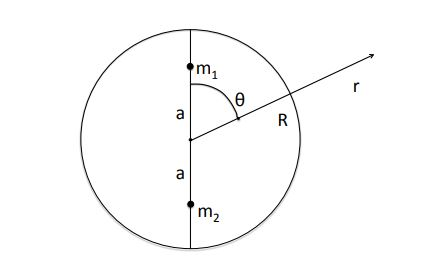
\includegraphics[width=\linewidth]{planetfigure.JPG}
        
        \item Assuming $r \gg R>a$, write $\phi(r,\theta)$ as a series in Legendre polynomials. Keep the first three leading terms. Check if your result matches solution of Laplace's equation, {\bf LP}, eq.  (37) (see also {\bf LP} eq.   (34) and related text).  
        
        \item Does your result match the measurement?  For what parameters?  Comment as adequate: can you exclude the existence of the two military bases?
        
      \end{enumerate}
    
  \end{enumerate}
  % End of Problem set on special functions

  \pagebreak

  \textbf{Exercises set on special functions} (5 points)
  \begin{enumerate}
    \item Using the method discussed in class 16, show that the equations below can be solved in terms of Bessel functions, and find their general solution.
    
    \begin{enumerate}
    \item $y^{\prime \prime }+2n^{2}xy=0$
    
    \item $xy^{\prime \prime }+\left( 2n+1\right) y^{\prime }+xy=0$
    \end{enumerate}
    
    
    
    \item Consider the generating function of Bessel functions, $G(x,h)$. Show that $G\left( x+y,\,h\right) =G\left( x,\,h\right) G\left(
    y,\,h\right) .$

      \textcolor{hwColor}{
        From page 612 of the textbook we learned that, the Bessel fuctions $\mathcal{J}_v(x)$, where $v=n$ is an integer,
        can be described by a generating function in a way similar to that discussed for Legendre polynomials. The genrerating 
        function for Bessel functions of integer order is given by 
        $$\mathcal{G}(x,h)=exp \left[\dfrac{x}{2}(h-\dfrac{1}{h})\right]=\sum\limits_{n=-\infty}^{\infty}\mathcal{J}_n(x) h^n$$ 
        Hence we have the following: 
        \\
        \\
        $
          \mathcal{G}(x+y, h)= exp\left[\dfrac{x+y}{2} \left(h-\dfrac{1}{h}\right)\right]
          \\
          \\
          =exp \left[\dfrac{x}{2} \left(h-\dfrac{1}{h}\right)+\dfrac{y}{2} \left(h-\dfrac{1}{h}\right)\right]
          \\
          \\
          =exp \left[\dfrac{x}{2} \left(h-\dfrac{1}{h}\right)\right]+exp \left[\dfrac{y}{2} \left(h-\dfrac{1}{h}\right)\right]
          \\
          \\
          \therefore ~~~ \mathcal{G}(x+y, h)=\mathcal{G}(x,h) \mathcal{G}(y,h)
        $
      }
    
    \item Use the result in the previous exercise to show that $J_{m}\left( x+y\right) =\sum\limits_{k=-\infty}^{\infty }J_{k}\left( x\right) J_{m-k}\left( y\right) .$
    
    
    \item Express each of the following in terms of Legendre polynomials, $
    P_{n}\left( x\right) $:

      \textcolor{hwColor}{
        We have $$P_n(x)=\dfrac{1}{2^n n!} \dfrac{d^n}{dx^n} (x^2-1)^n$$
        With the help of the above formula we have: \\
        \\
        $
          \begin{cases}
            P_0(x)=1
            \\
            P_1(x)=x
            \\
            P_2(x)=\dfrac{1}{2} (3x^2-1)
            \\
            P_3(x)=\dfrac{1}{2} (5x^3-3x)
            \\
            P_4(x)=\dfrac{1}{8} (35x^4-30x^2+3)
          \end{cases} \Longrightarrow \begin{cases}
            x=P_1
            \\
            x^2=\dfrac{2P_2+1}{3}
            \\
            x^3=\dfrac{2}{5} P_3+\dfrac{3}{5}x=\dfrac{2}{5} P_3+\dfrac{3}{5}P_1
            \\
            x^4=\dfrac{8P_4+30x^2-3}{35} 
            \\
            =\dfrac{8P_4+30\left(\dfrac{2P_2+1}{3}\right)-3}{35}
            \\
            =\dfrac{8P_4+20P_2+7}{35} 
          \end{cases}
        $
      }
      
      \begin{enumerate}
        \item $x-x^{3}$
        
          \textcolor{hwColor}{
            $
              f(x)=x-x^3=P_1-\dfrac{2}{5} P_3+\dfrac{3}{5}P_1
              \\
              \\
              \therefore ~~~~ f(x)=\dfrac{2}{5} P_1-\dfrac{2}{5}P_3
            $ 
          }
        
        \item $7x^{4}-3x+1$
        
          \textcolor{hwColor}{
            $
              f(x)=7x^{4}-3x+1=7\left(\dfrac{8P_4+20P_2+7}{35}\right)-3P_1+1
              \\
              \\
              \therefore ~~~~ f(x)=\dfrac{12}{5}P_0-3P_1+4P_2+\dfrac{8}{5}P_4
            $
          }

      \end{enumerate}
    
    \item Use the generating function for Legendre polynomials to obtain $P_{3}\left(x\right)$.
    
    \item Use the Rodrigues formula for Legendre polynomials to obtain $P_{4}\left(x\right)$.
    
    
    \item Write the delta function, $\delta \left( x\right)$, as a series in Legendre polynomials over the range \newline $-1\leq x\leq 1$.
    
    
    \item Write each of the following expressions as spherical harmonics (do not forget the normalization factors and powers of $r$) where $x$, $y$, and $z$ are the Cartesian coordinate variables:
    
      \begin{enumerate}
      
        \item $x^{2}-y^{2}$
        
        \item $z$
        
        \item $z^{2}$
        
        \item $x^{2}-2ixy+y^{2}$
        
        \item $xyz$
      \end{enumerate}
    
  \end{enumerate}
  % End of Exercises set on special functions

  \pagebreak

  \textbf{Exercises set on Analytic functions} (5 points)
  \begin{enumerate}

    \item  Given the following functions, determine first if each is harmonic, and if so, find an analytic function that has it as its real part, $u(x,y)$. Express each analytic function in terms of $z$.
    
    \begin{enumerate}
    
      \item $e^{x}\cos x$
      
      \item $2x\left( 3+y\right)$
      
      \item $x^{2}+y^{2}$
    \end{enumerate}
    
    
    \item Evaluate the following integrals:
    
    \begin{enumerate}
    
    \item  (5 points total including all the different contours)
    \[
    \oint_{C}\frac{\sin 2z}{z^{2}-4z+5}\,dz
    \]
    
    \begin{enumerate}
      \item where $C$ is the circle $\left| z\right| =1.$
      
      \item where $C$ is the circle $\left| z-2i\right| =3.$
      
      \item where $C$ is the circle $\left| z-1+2i\right| =2.$
    \end{enumerate}
    
    \item   (5 points total including all the different contours)
    \[
    \oint_{C}\frac{e^{z}}{\left( z+1\right) ^{2}}\,dz
    \]
    
      \begin{enumerate}
        \item where $C$ is the circle $\left| z-1\right| =3.$
        
        \item where $C$ is the circle $\left| z-1\right| =1.$
        
        \item where $C$ is the circle $\left| z-2i\right| =3.$
      \end{enumerate}
    \end{enumerate}
    
    
    \item Find the Laurent series for each of the following functions about the point and in the region(s) indicated.
    
    \begin{enumerate}
      \item $f\left( z\right) =\frac{\displaystyle z}{\displaystyle z^{2}-5z+6}$; $z_{0}=2$; $0 \leq \left|z-2\right| <1$
      
      \item $f\left( z\right) =\frac{\displaystyle z}{\displaystyle z^{2}-5z+6}$; $z_{0}=2$; $1<\left| z-2\right| <\infty $.
      
      \item $f\left( z\right) =\frac{\displaystyle z^{2}}{\displaystyle z^{2}+1}$, $z_{0}=$ $1$; $0 \leq \left| z-1\right| <\sqrt{2}$.
      
      \item $f\left( z\right) =\frac{\displaystyle z^{2}}{\displaystyle z^{2}+1}$, $z_{0}=$ $1$;  $\left| z-1\right| >\sqrt{2}$.
      
      
      \item $f\left( z\right) =\frac{\displaystyle e^{z}-1}{\displaystyle z^{2}}$, $z_{0}=0$, $0<\left|
      z\right| <\infty $.
    
    
    \end{enumerate}
    
    \item Find the residues of the given functions at all of their poles:
    
    \begin{enumerate}
  
      \item \[
      f\left( z\right) =\frac{1+z}{1-\cos z}
      \]
      
      \item \[
      f\left( z\right) =\frac{z^{2}}{\left( z^{2}+3z+2\right) ^{2}}
      \]
      
      \item \[
      f\left( z\right) =\frac{\ln z}{1+z^{2}},\;-\pi <\arg \left( z\right) \leq \pi.
      \]
    \end{enumerate}
    
    \item Compute the following integrals using residues:
    
    \begin{enumerate}
      \item \[
      \oint_{C}\frac{z}{z^{2}-1}\,dz;\hspace{0.2in}C:\;\left| z\right| =4
      \]
      
      \item \[
      \oint_{C}\tan z\,\,dz;\hspace{0.2in}C:\;\left| z\right| =2
      \]
      
      \item \[
      \oint_{C}\frac{1+z}{1-\cos z}\,dz;\hspace{0.2in}C:\;\left| z\right| =8
      \]
      
      \item \[
      \oint_{C}\frac{1}{z^{2}+z+1}\,dz;\hspace{0.2in}C:\;\left| z-1\right| =\frac{3}{2}
      \]
    \end{enumerate}
    
    \item Compute the following integrals using residues:
    
    \begin{enumerate}
      \item \[
      \int_{0}^{2\pi }\frac{d\theta }{5+3\cos \theta }
      \]
      
      \item \[
      \int_{0}^{\infty }\frac{x\sin x}{1+x^{2}}\,dx
      \]
    \end{enumerate}
    
  
    \end{enumerate}
  % End of Exercises set on Analytic functions

\end{document}